% Author: Naomi Sagan, Ryan Koh
% Emails: naomi.sagan@berkeley.edu, ryan_koh@berkeley.edu

\qns{Intro to Discrete-Time Systems}

\usetikzlibrary{calc, automata, chains, arrows.meta}

Students are studying for the EECS16C exam, and the flow of students from Moffit to Taejin's Office Hours (OH) can be represented as the following: \newline

\begin{align*}
    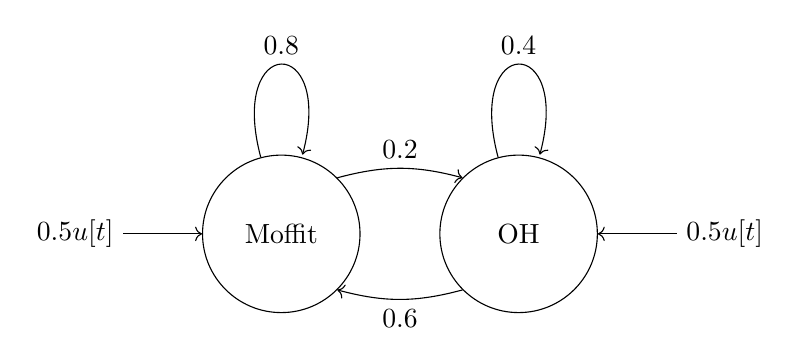
\begin{tikzpicture}
        \node[circle, draw=black, minimum size=2cm] (Moffit) {Moffit};
        \node[circle, draw=black, minimum size=2cm] (OH) [right=of Moffit] {OH};
        \draw [->] (Moffit.north east) to [bend left=15]  node[above] {0.2}  (OH.north west);
        \path (Moffit) edge [loop above] node {0.8} (Moffit);
        \path (OH) edge [loop above] node {0.4} (OH);
        \node (u_moffit) [left=of Moffit] {$0.5u[t]$};
        \draw [->] (u_moffit.east) to []  node[left] {}  (Moffit.west);
        \node (u_OH) [right=of OH] {$0.5u[t]$};
        \draw [->] (u_OH.west) to []  node[right] {}  (OH.east);
        \draw [->] (OH.south west) to [bend left=15] node[below] {0.6} (Moffit.south east);
    \end{tikzpicture}
\end{align*}

where $u[t]$ is the number of students that start to study at timestep $t$. (i.e.: $u[t]$ is the input to the system)

\begin{enumerate}
    \qitem Let our state variables be represented by $x_1$ and $x_2$. \textbf{Explain in your own words what the state variables $x_1$ and $x_2$ could represent in our system}
        \sol{
            We can represent our state by the number of students in Moffit ($x_1$) and the number of students in Taejin's office hours ($x_2$).
        }
    \ws{\vspace{2.5cm}}
    \qitem Represent the flow of students between the two states as a matrix-vector discrete time system:
    \begin{align*}
        \vec{x}[t+1] =  A\vec{x}[t] + \vec{b}u[t]\\
    \end{align*}
    \textbf{Find matrix $A$ and vector $\vec{b}$.} \\
    \sol{
        \begin{align*}
            \begin{bmatrix}
                x_1[t + 1] \\ x_2[t + 1]
            \end{bmatrix} =
            \begin{bmatrix}
                0.8 & 0.6 \\
                0.2 & 0.4
            \end{bmatrix}
            \begin{bmatrix}
                x_1[t] \\ x_2[t]
            \end{bmatrix} +
            \begin{bmatrix}
                0.5 \\ 0.5
            \end{bmatrix} u[t]
        \end{align*}
    }
    \ws{\vspace{8cm}}
    \qitem Let $\vec{x}[0] = \vec{0}$, and $u[t] = 10$ for all values of $t$. \textbf{What is $\vec{x}[1]$? What is $\vec{x}[2]$?} \textbf{What is $||\vec{x}||$ as $t\rightarrow\infty$? Does that make sense in the context of our problem?}

    \sol{
        \begin{align*}
            \vec{x}[1] = A \vec{0} + 10
            \begin{bmatrix}
                0.5 \\ 0.5
            \end{bmatrix} =
            \begin{bmatrix}
                5 \\ 5
            \end{bmatrix} \\
            \vec{x}[2] = A
            \begin{bmatrix}
                5 \\ 5
            \end{bmatrix} + 10
            \begin{bmatrix}
                0.5 \\ 0.5
            \end{bmatrix} =
            \begin{bmatrix}
                0.8 & 0.6 \\
                0.2 & 0.4
            \end{bmatrix}
            \begin{bmatrix}
                5 \\ 5
            \end{bmatrix} +
            \begin{bmatrix}
                5 \\ 5
            \end{bmatrix} =
            \begin{bmatrix}
                12 \\ 8
            \end{bmatrix}
        \end{align*}

        The input to the system is always positive, and no students ever leave the system, so the magnitude of the state keeps on growing. So,
        \begin{align*}
            \lim_{t \to \infty} ||\vec{x}[t]|| = \infty
        \end{align*}
        This does not make sense in the context of our problem because it is impossible to have an infinite amount of students.
    }

    \ws{\vspace{8cm}}
    \qitem Let $\vec{x}[0] = \begin{bmatrix} 50 \\ 50 \end{bmatrix}$, and $u[t] = -4$ for all values of $t$. \textbf{What is $\vec{x}[1]$? What is $\vec{x}[2]$?} \textbf{What is $||\vec{x}||$ as $t\rightarrow\infty$? What sign are the elements of $\vec{x}$? Does that make sense in the context of our problem?}

\sol{
        \begin{align*}
            \vec{x}[1] = A
            \begin{bmatrix}
                50 \\ 50
            \end{bmatrix} - 4
            \begin{bmatrix}
                0.5 \\ 0.5
            \end{bmatrix} =
            \begin{bmatrix}
                0.8 & 0.6 \\
                0.2 & 0.4
            \end{bmatrix}
            \begin{bmatrix}
                50 \\ 50
            \end{bmatrix} -
            \begin{bmatrix}
                2 \\ 2
            \end{bmatrix} =
            \begin{bmatrix}
                68 \\ 28
            \end{bmatrix} \\
            \vec{x}[2] = A
            \begin{bmatrix}
                68 \\ 28
            \end{bmatrix} - 4
            \begin{bmatrix}
                0.5 \\ 0.5
            \end{bmatrix} =
            \begin{bmatrix}
                0.8 & 0.6 \\
                0.2 & 0.4
            \end{bmatrix}
            \begin{bmatrix}
                68 \\ 28
            \end{bmatrix} -
            \begin{bmatrix}
                2 \\ 2
            \end{bmatrix}  =
            \begin{bmatrix} 69.2 \\ 22.8 \end{bmatrix}
        \end{align*}
        It's ok that the state variables are not whole numbers! Think of them as the average number of students in Moffit and Taejin's OH.
        \newline
        The input to the system is always negative, and no students are ever added to the system, so the magnitude of the state keeps on decreasing linearly. So, \textbf{the sign of the elements of $\vec{x}$ is negative} and
        \begin{align*}
            \lim_{t \to \infty} ||\vec{x}[t]|| = \infty
        \end{align*}
        This does not make sense in the context of our problem because there is an infinitely negative amount of students in our system.
    }

    \ws{\vspace{12cm}}
    \qitem Let $\vec{x}[0] = \vec{0}$, $u[0] = 16$, and $u[t>0] = 0$. \textbf{What is $\vec{x}[1]$? What is $\vec{x}[2]$?} \textbf{What is the largest $||\vec{x}||$ can get as $t\rightarrow\infty$? Does that make sense in the context of our problem?}

    \sol {
        \begin{align*}
            \vec{x}[1] = A \vec{0} + 16
            \begin{bmatrix}
                0.5 \\ 0.5
            \end{bmatrix} =
            \begin{bmatrix}
                8 \\ 8
            \end{bmatrix} \\
            \vec{x}[2] = A
            \begin{bmatrix}
                8 \\ 8
            \end{bmatrix} + 0
            \begin{bmatrix}
                0.5 \\ 0.5
            \end{bmatrix} =
            \begin{bmatrix}
                0.8 & 0.6 \\
                0.2 & 0.4
            \end{bmatrix}
            \begin{bmatrix}
                8 \\ 8
            \end{bmatrix} =
            \begin{bmatrix} 11.2 \\ 4.8 \end{bmatrix}
        \end{align*}

        The input to the system is 0 after the first time step, and the sum of students in the two states stays the same each timestep, so, by the triangle inequality, the magnitude of $\vec{x}$ will remain less than or equal to the sum of the students in the two states after the first timestep.
        \begin{align*}
            \lim_{t \to \infty} ||\vec{x}[t]|| \leq 16
        \end{align*}
        This \textit{does} make sense in the context of our problem because it is a finite, positive number.
    }

\end{enumerate}
